% Options for packages loaded elsewhere
\PassOptionsToPackage{unicode}{hyperref}
\PassOptionsToPackage{hyphens}{url}
%
\documentclass[
]{article}
\usepackage{amsmath,amssymb}
\usepackage{iftex}
\ifPDFTeX
  \usepackage[T1]{fontenc}
  \usepackage[utf8]{inputenc}
  \usepackage{textcomp} % provide euro and other symbols
\else % if luatex or xetex
  \usepackage{unicode-math} % this also loads fontspec
  \defaultfontfeatures{Scale=MatchLowercase}
  \defaultfontfeatures[\rmfamily]{Ligatures=TeX,Scale=1}
\fi
\usepackage{lmodern}
\ifPDFTeX\else
  % xetex/luatex font selection
\fi
% Use upquote if available, for straight quotes in verbatim environments
\IfFileExists{upquote.sty}{\usepackage{upquote}}{}
\IfFileExists{microtype.sty}{% use microtype if available
  \usepackage[]{microtype}
  \UseMicrotypeSet[protrusion]{basicmath} % disable protrusion for tt fonts
}{}
\makeatletter
\@ifundefined{KOMAClassName}{% if non-KOMA class
  \IfFileExists{parskip.sty}{%
    \usepackage{parskip}
  }{% else
    \setlength{\parindent}{0pt}
    \setlength{\parskip}{6pt plus 2pt minus 1pt}}
}{% if KOMA class
  \KOMAoptions{parskip=half}}
\makeatother
\usepackage{xcolor}
\usepackage[margin=1in]{geometry}
\usepackage{graphicx}
\makeatletter
\def\maxwidth{\ifdim\Gin@nat@width>\linewidth\linewidth\else\Gin@nat@width\fi}
\def\maxheight{\ifdim\Gin@nat@height>\textheight\textheight\else\Gin@nat@height\fi}
\makeatother
% Scale images if necessary, so that they will not overflow the page
% margins by default, and it is still possible to overwrite the defaults
% using explicit options in \includegraphics[width, height, ...]{}
\setkeys{Gin}{width=\maxwidth,height=\maxheight,keepaspectratio}
% Set default figure placement to htbp
\makeatletter
\def\fps@figure{htbp}
\makeatother
\setlength{\emergencystretch}{3em} % prevent overfull lines
\providecommand{\tightlist}{%
  \setlength{\itemsep}{0pt}\setlength{\parskip}{0pt}}
\setcounter{secnumdepth}{-\maxdimen} % remove section numbering
\ifLuaTeX
  \usepackage{selnolig}  % disable illegal ligatures
\fi
\usepackage{bookmark}
\IfFileExists{xurl.sty}{\usepackage{xurl}}{} % add URL line breaks if available
\urlstyle{same}
\hypersetup{
  pdftitle={9. Appendices},
  pdfauthor={B233241},
  hidelinks,
  pdfcreator={LaTeX via pandoc}}

\title{9. Appendices}
\author{B233241}
\date{2025-01-07}

\begin{document}
\maketitle

\subsection{Appendix A: List of
Abbreviations}\label{appendix-a-list-of-abbreviations}

\subsection{Appendix B: Simulation
Code}\label{appendix-b-simulation-code}

\subsubsection{Generating Data and
Models}\label{generating-data-and-models}

The data generating model used was from Appendix 3 of Bowden et al
(ref); the relevant section describing their model is reproduced below:

\_``\ldots{}

\begin{equation} 
U_i = \sum^J_{j=1} \phi_jG_{ij} + \epsilon_i^U
\end{equation}

\begin{equation} 
X_i = \sum^J_{j=1} \gamma_jG_{ij} + U_i + \epsilon_i^X
\end{equation}

\begin{equation} 
Y_i = \sum^J_{j=1} \alpha_jG_{ij} + \beta X_i + U_i + \epsilon_i^Y
\end{equation}

for participants indexed by \(i = 1, . . . , N\), and genetic
instruments indexed by \(j = 1, . . . , J\). The error terms
\(\epsilon_i^U , \epsilon_i^X\) and \(\epsilon_i^Y\) were each drawn
independently from standard normal distributions. The genetic effects on
the exposure γj are drawn from a uniform distribution between 0.03 and
0.1. Pleiotropic effects \(\alpha_j\) and \(\phi_j\) were set to zero if
the genetic instrument was a valid instrumental variable. Otherwise
(with probability 0.1, 0.2, or 0.3):

\begin{enumerate}
\def\labelenumi{\arabic{enumi}.}
\item
  In Scenario 1 (balanced pleiotropy, InSIDE satisfied), the
  \(\alpha_j\) parameter was drawn from a uniform distribution between
  −0.2 and 0.2.
\item
  In Scenario 2 (directional pleiotropy, InSIDE satisfied), the
  \(\alpha_j\) parameter was drawn from a uniform distribution between 0
  and 0.2.
\item
  In Scenario 3 (directional pleiotropy, InSIDE not satisfied), the
  \(\phi_j\) parameter was drawn from a uniform distribution between
  −0.2 and 0.2.
\end{enumerate}

The causal effect of the exposure on the outcome was either
\(\beta X = 0\) (null causal effect) or \(\beta X = 0.1\) (positive
causal effect). A total of 10 000 simulated datasets were generated for
sample sizes of N = 10 000 and 20 {[}sic{]} participants. Only the
summary data, that is genetic associations with the exposure and with
the outcome and their standard errors as estimated by univariate
regression on the genetic instruments in turn, were used by the analysis
methods. In the two-sample setting, data were generated on 2N
participants, and genetic associations with the exposure were estimated
in the first N participants, and genetic associations with the outcome
in the second N participants.''\_ (ref)

To reproduce this model, code was written in R to generate the relevant
participant level data. First, a function (`simulate\_MR\_data) was
written which included parameters specified by Bowden et al, and also to
allow testing of data simulation:

This initial simulation function generated data in the following format:

\begin{verbatim}
## List of 10
##  $ U           :List of 2
##   ..$ : num [1:2000, 1] 0 0 0 0 0 0 0 0 0 0 ...
##   ..$ : num [1:2000, 1] 0 0 0 0 0 0 0 0 0 0 ...
##  $ X           :List of 2
##   ..$ : num [1:1000, 1] 1.12 1.59 1.76 1.49 1.56 ...
##   ..$ : num [1:1000, 1] 1.84 1.7 1.6 1.66 1.5 ...
##  $ Y           :List of 2
##   ..$ : num [1:1000, 1] -0.24 -0.311 -0.393 -0.227 -0.1 ...
##   ..$ : num [1:1000, 1] -0.872 -0.901 -0.772 -0.999 -0.477 ...
##  $ G_X         :List of 2
##   ..$ : int [1:1000, 1:25] 0 1 1 1 1 0 0 0 0 0 ...
##   ..$ : int [1:1000, 1:25] 1 2 1 2 2 2 2 2 2 2 ...
##  $ G_Y         :List of 2
##   ..$ : int [1:1000, 1:25] 0 1 1 0 1 0 0 0 0 0 ...
##   ..$ : int [1:1000, 1:25] 2 2 2 2 1 2 1 1 2 1 ...
##  $ alpha       :List of 2
##   ..$ : num [1:25] -0.106 0 -0.121 0 0 ...
##   ..$ : num [1:25] 0 0 -0.0786 0 0 ...
##  $ gamma       :List of 2
##   ..$ : num [1:25] 0.0902 0.0878 0.08 0.0832 0.084 ...
##   ..$ : num [1:25] 0.0374 0.0721 0.0975 0.085 0.0322 ...
##  $ phi         :List of 2
##   ..$ : num [1:25] 0 0 0 0 0 0 0 0 0 0 ...
##   ..$ : num [1:25] 0 0 0 0 0 0 0 0 0 0 ...
##  $ beta        :List of 2
##   ..$ : num 0.1
##   ..$ : num 0.1
##  $ prop_invalid:List of 2
##   ..$ : num 0.3
##   ..$ : num 0.3
\end{verbatim}

A function (\texttt{extract\_models}) was then written to create linear
models from each dataset generated as per Bowden et al:

This model generated estimates of the coefficient of gene:exposure
association (\texttt{coeff\_G\_X}), coefficient of gene:outcome
association (\texttt{coeff\_G\_Y}), and the relevant standard errors of
these estimates. The values of parameters inputted were also returned to
aid in further testing of data/model generation, i.e.~actual
gene:exposure associations (\texttt{gamma}), pleiotropic effects of
invalid instruments (\texttt{alpha}), additional pleiotropic effects
when InSIDE assumption not satified (\texttt{phi}), causal effect of
exposure on outcome (\texttt{beta}) and the proportion of invalid
genetic instruments with pleiotropic effects on the outcome
(\texttt{prop\_invalid}).

\begin{verbatim}
##     dataset    Instrument   coeff_G_X        coeff_G_X_SE      
##  Min.   :1   Min.   : 1   Min.   :0.03006   Min.   :1.591e-16  
##  1st Qu.:1   1st Qu.: 7   1st Qu.:0.03791   1st Qu.:1.702e-16  
##  Median :1   Median :13   Median :0.05578   Median :1.847e-16  
##  Mean   :1   Mean   :13   Mean   :0.06018   Mean   :2.346e-16  
##  3rd Qu.:1   3rd Qu.:19   3rd Qu.:0.07998   3rd Qu.:2.441e-16  
##  Max.   :1   Max.   :25   Max.   :0.09140   Max.   :7.259e-16  
##      gamma           coeff_G_Y           coeff_G_Y_SE           alpha          
##  Min.   :0.03006   Min.   :-0.1188256   Min.   :0.0009824   Min.   :-0.120669  
##  1st Qu.:0.03791   1st Qu.: 0.0006676   1st Qu.:0.0010520   1st Qu.: 0.000000  
##  Median :0.05578   Median : 0.0031161   Median :0.0011837   Median : 0.000000  
##  Mean   :0.06018   Mean   :-0.0047291   Mean   :0.0014576   Mean   :-0.008692  
##  3rd Qu.:0.07998   3rd Qu.: 0.0068099   3rd Qu.:0.0015114   3rd Qu.: 0.000000  
##  Max.   :0.09140   Max.   : 0.1356693   Max.   :0.0040567   Max.   : 0.133513  
##       phi         beta      prop_invalid
##  Min.   :0   Min.   :0.1   Min.   :0.3  
##  1st Qu.:0   1st Qu.:0.1   1st Qu.:0.3  
##  Median :0   Median :0.1   Median :0.3  
##  Mean   :0   Mean   :0.1   Mean   :0.3  
##  3rd Qu.:0   3rd Qu.:0.1   3rd Qu.:0.3  
##  Max.   :0   Max.   :0.1   Max.   :0.3
\end{verbatim}

\subsubsection{Testing Generation of Data and
Models}\label{testing-generation-of-data-and-models}

A series of test plots were used to verify that data were simulated as
intended under the various conditions specified by input parameters.
Test plots were not created for the parameters \texttt{n\_participants},
\texttt{n\_instruments} or \texttt{n\_datasets}, as the functioning of
these parameters could be readily inferred from the datasets outputted,
as above.

The \texttt{prop\_invalid} parameter specifies the proportion of invalid
genetic instruments simulated, i.e.~the proportion of genetic
instruments affecting the outcome via direct/pleiotropic effects, and
thus not solely via the exposure of interest. If simulated correctly,
increasing the value of \texttt{prop\_invalid} should increase the
number of instruments with pleiotropic effects, i.e.~instruments with
\texttt{alpha} =/= 0.

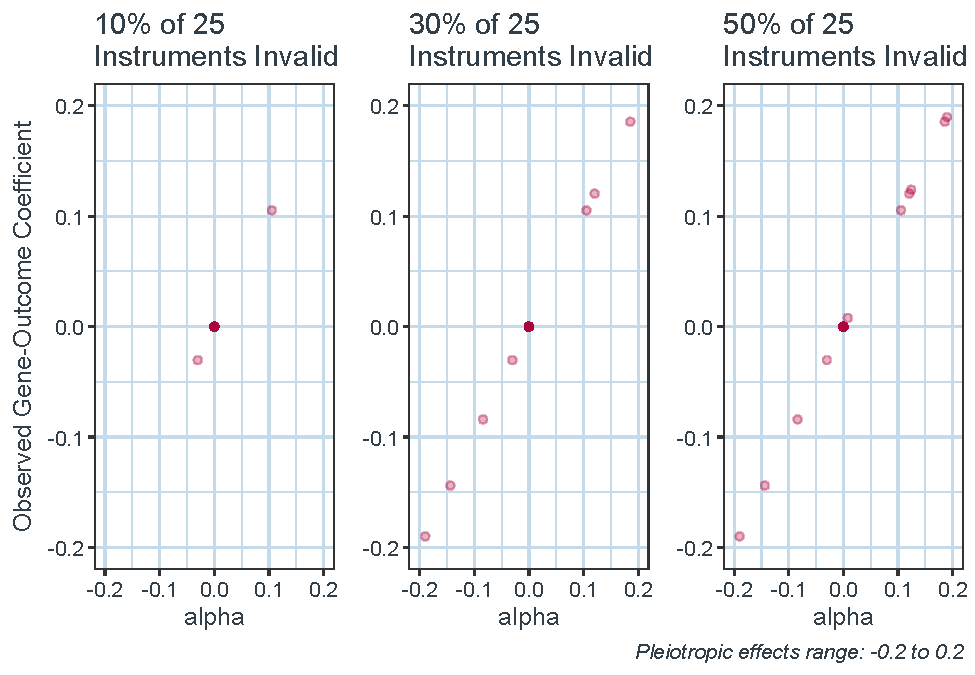
\includegraphics{C:/Users/timol/OneDrive/Documents/R/WORKIN~1/DATA_S~1/Dissertation_Bayes_MR/MSc_Thesis/MSc_Thesis_Split/Output_9_Appendices_files/figure-latex/test-plot-prop-invalid-1.pdf}
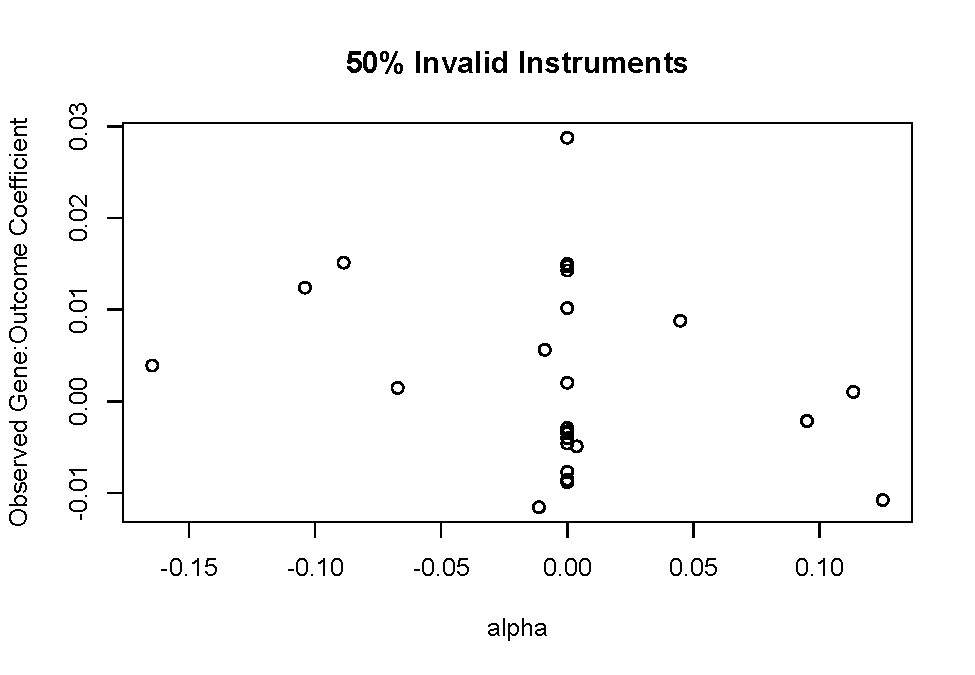
\includegraphics{C:/Users/timol/OneDrive/Documents/R/WORKIN~1/DATA_S~1/Dissertation_Bayes_MR/MSc_Thesis/MSc_Thesis_Split/Output_9_Appendices_files/figure-latex/test-plot-prop-invalid-2.pdf}

\begin{verbatim}
## 
## CHECKING DATA AND PREPROCESSING FOR MODEL 'MRHevo.summarystats' NOW.
## 
## COMPILING MODEL 'MRHevo.summarystats' NOW.
## 
## STARTING SAMPLER FOR MODEL 'MRHevo.summarystats' NOW.
\end{verbatim}

\begin{verbatim}
## # A tibble: 1 x 19
##   WME_est WME_se WME_pval WME_Q WME_Q_df WME_Q_pval WME_nsnp Hevo_est Hevo_se
##     <dbl>  <dbl>    <dbl> <dbl>    <dbl>      <dbl>    <int>    <dbl>   <dbl>
## 1  -0.124 0.0911    0.173    NA       NA         NA       25  -0.0753 0.00111
## # i 10 more variables: Hevo_sd <dbl>, Hevo_2.5 <dbl>, Hevo_25 <dbl>,
## #   Hevo_50 <dbl>, Hevo_75 <dbl>, Hevo_97.5 <dbl>, Hevo_n_eff <dbl>,
## #   Hevo_n_Rhat <dbl>, Hevo_z_stat <dbl>, Hevo_pval <dbl>
\end{verbatim}

\subsection{Citation Search Strategy}\label{citation-search-strategy}

\end{document}
